\documentclass[tikz,border=8pt]{standalone}
\usepackage{tikz}
\usepackage{helvet}
\renewcommand{\familydefault}{\sfdefault}
\usetikzlibrary{positioning,arrows.meta,fit,backgrounds,calc}

\begin{document}
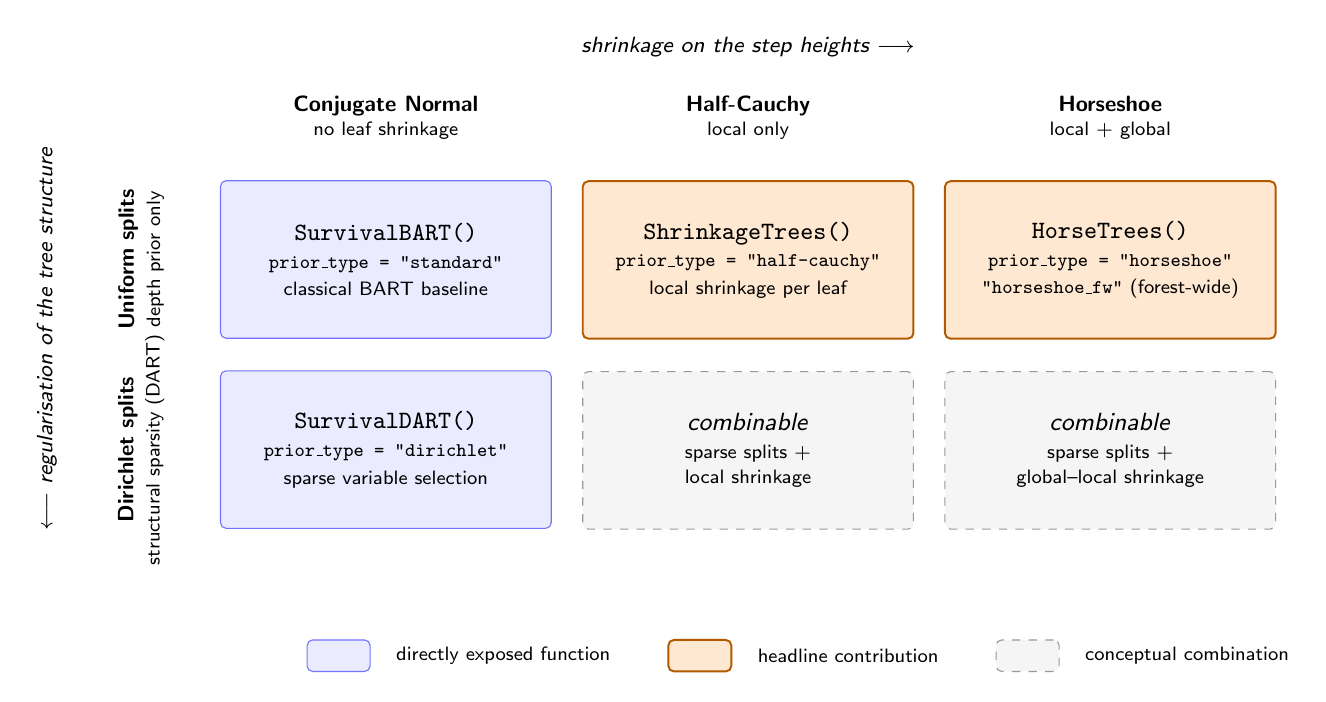
\begin{tikzpicture}[
  font=\small,
  >={Stealth[length=2.4mm,width=1.8mm]},
  cell/.style={
    draw=black!55, rounded corners=2pt, align=center,
    minimum width=42mm, minimum height=20mm,
    inner sep=3pt, fill=white
  },
  % Filled: directly available through the package API
  filled/.style={cell, fill=blue!8,  draw=blue!55},
  % Key: the package's novel contribution
  key/.style   ={cell, fill=orange!18, draw=orange!70!black, line width=0.7pt},
  % Combo: reachable conceptually but not through a single named wrapper
  combo/.style ={cell, fill=black!4,  draw=black!40, dashed},
  collabel/.style={font=\bfseries\footnotesize, align=center},
  rowlabel/.style={font=\bfseries\footnotesize, align=center, rotate=90},
  axislabel/.style={font=\itshape\footnotesize, align=center},
  title/.style={font=\bfseries}
]

% ---------- Column headers (step-height prior) ----------
\node[collabel] (h1) at (0,0)   {Conjugate Normal\\[-1pt]{\normalfont\scriptsize no leaf shrinkage}};
\node[collabel] (h2) at (4.6,0) {Half-Cauchy\\[-1pt]{\normalfont\scriptsize local only}};
\node[collabel] (h3) at (9.2,0) {Horseshoe\\[-1pt]{\normalfont\scriptsize local $+$ global}};

% ---------- Row 1: Uniform splits ----------
\node[filled, below=4mm of h1] (c11) {%
  \texttt{SurvivalBART()}\\[-1pt]
  \scriptsize \texttt{prior\_type = "standard"}\\[-1pt]
  \scriptsize classical BART baseline};

\node[key, below=4mm of h2] (c12) {%
  \texttt{ShrinkageTrees()}\\[-1pt]
  \scriptsize \texttt{prior\_type = "half-cauchy"}\\[-1pt]
  \scriptsize local shrinkage per leaf};

\node[key, below=4mm of h3] (c13) {%
  \texttt{HorseTrees()}\\[-1pt]
  \scriptsize \texttt{prior\_type = "horseshoe"}\\[-1pt]
  \scriptsize \texttt{"horseshoe\_fw"} (forest-wide)};

% ---------- Row 2: Dirichlet splits ----------
\node[filled, below=4mm of c11] (c21) {%
  \texttt{SurvivalDART()}\\[-1pt]
  \scriptsize \texttt{prior\_type = "dirichlet"}\\[-1pt]
  \scriptsize sparse variable selection};

\node[combo,  below=4mm of c12] (c22) {%
  \emph{combinable}\\[-1pt]
  \scriptsize sparse splits $+$\\[-2pt]
  \scriptsize local shrinkage};

\node[combo,  below=4mm of c13] (c23) {%
  \emph{combinable}\\[-1pt]
  \scriptsize sparse splits $+$\\[-2pt]
  \scriptsize global--local shrinkage};

% ---------- Row labels (splitting rule) ----------
\node[rowlabel] at ($(c11.west)+(-1.0,0)$)
      {Uniform splits\\{\normalfont\scriptsize depth prior only}};
\node[rowlabel] at ($(c21.west)+(-1.0,0)$)
      {Dirichlet splits\\{\normalfont\scriptsize structural sparsity (DART)}};

% ---------- Axis labels ----------
\node[axislabel] at ($(h2)+(0,0.9)$) {shrinkage on the step heights $\longrightarrow$};
\node[axislabel, rotate=90] at ($(c21.west)+(-2.2,1.4)$)
     {$\longleftarrow$ regularisation of the tree structure};

% ---------- Legend (centred below the middle column) ----------
\begin{scope}[shift={($(c22.south)+(-5.2,-1.6)$)}]
  \node[filled, minimum width=8mm, minimum height=4mm, inner sep=0pt] (lk1) {};
  \node[right=2mm of lk1, font=\scriptsize] (lk1t) {directly exposed function};
  \node[key,    right=6mm of lk1t, minimum width=8mm, minimum height=4mm, inner sep=0pt] (lk2) {};
  \node[right=2mm of lk2, font=\scriptsize] (lk2t) {headline contribution};
  \node[combo,  right=6mm of lk2t, minimum width=8mm, minimum height=4mm, inner sep=0pt] (lk3) {};
  \node[right=2mm of lk3, font=\scriptsize] {conceptual combination};
\end{scope}

\end{tikzpicture}
\end{document}
